\csname documentclass\endcsname[../main.tex]{subfiles}
\begin{document}
\chapter{Method}\label{chapter-3}


In this chapter, we propose 
to learn a non-greedy intervention policy using Reinforcement Learning.
We first
formalise interventions and intervention policies,
we then formulate the problem of 
finding concepts to intervene on for a budget as a Reinforcement Learning problem. We introduce
the surrogate models we use
to calculate intermediate rewards,
and finally, present how Reinforcement Learning is used 
to learn a non-greedy intervention policy.

Building on top of IntCEMs, which augment a CEM
with a greedy intervention policy model and train the two simultaneously,
we propose RLCEM,
a novel CEM model augmented with a Reinforcement Learning agent
that learns a non-greedy intervention policy.
The CEM and RL agent are trained simultaneously, similar to IntCEM, 
where the sampled interventions are used to increase the
$\mathbf{c} \to \mathbf{y}$ label predictor model's sensitivity to interventions. Additionally, we use an AC Flow model as a surrogate model to provide
intermediate rewards to the RL agent.


\section{Non-greedy Intervention Policies}
\label{method:non-greedy-policies}

Compared to a greedy intervention policy
defined in ~\ref{equation:greedy-intervention-policy}, for input predicted concept probabilities
$\hat{\mathbf{p}}$
, a non-greedy intervention 
policy $\mathcal{P}$ outputs a set of concepts to intervene on for a budget $j$, as defined in~\ref{equation:non-greedy-policies}
\begin{equation}\label{equation:non-greedy-policies}
\mathcal{P}(\hat{\mathbf{p}}, j) = \bm{\mu}, \quad \sum_{i=0}^k \mu_i \leq j
\end{equation}
Since we want the intervention policy to maximise 
the post-intervention accuracy of the $\mathbf{c} \to \mathbf{y}$ model, this is equivalent to maximising 
the function
\begin{equation}\label{equation:non-greedy-policies}
\hat{\mathcal{P}} = \mathop{\mathrm{argmax}}_{\mathcal{P}} \sum_{j=1}^k Acc(\hat{g}(\hat{\mathbf{c}}_{\mathcal{P}_j}), \mathbf{y}) 
\end{equation}
Where $\hat{\mathbf{c}}_{\mathcal{P}, j}$ is the predicted concepts after intervening using policy $\mathcal{P}$ and budget $j$.
\begin{equation}\label{equation:non-greedy-policies-max-2}
\hat{\mathbf{c}}_{\mathcal{P}, j} = I(\hat{\mathbf{c}}, \mathbf{c}, \mathcal{P}(\hat{\mathbf{c}}, j))
\end{equation}
However, in practice the intervention policy
contains more inputs such as the state of the CBM, as defined in Section~\ref{method:rl}.
Note that the notion of a budget, defined as the number
of concepts the model is allowed to intervene on for simplicity, is only
meaningful for non-greedy policies. Non-greedy policies aim
to maximise the accuracy of the $\mathbf{c} \to \mathbf{y}$ model after using up the intervention budget,
and may select different sets of intervention concepts 
for different budgets. Greedy policies always select the same
concepts per step and thus the budget does not 
affect the concept selected by the policy.
Thus, existing intervention policies are suboptimal for finding intervention policies 
with budgets.
% This is why existing intervention policies do not consider
% budgets, and why we consider them in our research question.

\subsection{Optimal Policy}
To show if non-greedy policies can outperform greedy policies, we conduct an
ablation study comparing two policies:
Greedy Optimal and True Optimal.
These are both the optimal policies that have access to the true label $\mathbf{y}$ during test time, which 
allows them to search and select the concepts
where intervening on these concepts yields a prediction
$\hat{\mathbf{y}} = \hat{g}(\hat{\mathbf{c}})$ 
with the highest accuracy.

While Greedy Optimal searches for 
the best concept group
out of all remaining un-intervened groups
to select at each step, True Optimal searches through
all possible combinations of concept groups to intervene at each budget, yielding
a time complexity of $O(n!)$ rather than
$O(n)$. This is why while IntCEM can 
learn a greedy intervention policy model directly
by training it to mimic the behaviour of a Greedy Optimal 
policy, it is infeasible to train a non-greedy intervention policy
model to mimic the behaviour of a True Optimal policy.

Greedy Optimal and True Optimal represent the theoretical
upper bound intervention performance
that greedy and non-greedy policies can achieve respectively,
and we compare the two to see if the optimal 
non-greedy intervention policy can outperform the 
optimal greedy
intervention policy.

As shown in Appendix~\ref{appendix:optimal-policies}, we show that True Optimal outperforms
Greedy Optimal in predictive accuracy after the same number of interventions.
 This shows that non-greedy policies 
can outperform greedy policies as they have a higher upper bound.



% Budget
% In this project, we utilize Reinforcement Learning

\section{Reinforcement Learning}\label{method:rl}
Following the success of using 
Reinforcement Learning to solve similar problems where we sequentially learn about the ground truth of concepts to improve final predictive accuracy~\cite{gsmrl,non-greedy-1},
we use Reinforcement Learning to learn a non-greedy intervention policy.

\subsection{Intermediate Rewards}

When learning a non-greedy policy, its performance is measured by the accuracy
of the model after all interventions in the end.
When training an RL agent to learn such a policy, this corresponds
to rewarding it at the final step based 
on the final accuracy, and training it to maximise this reward.
% if we were to train an RL agent by rewarding it in the intermediate steps
% this would become a greedy policy.
However, previous studies have shown that
using delayed rewards, where the agent is only rewarded after long episodes,
can pose a challenge to its learning as the agent struggles to learn
the consequences of its actions~\cite{ steps-towards-ai, temporal-credit-assignment},
and thus struggles to learn to make the correct decisions.

Therefore we introduce intermediate rewards 
to guide the RL agent to make the correct intermediate
interventions that lead 
to the largest final accuracy.
These intermediate rewards, similar to ECTP and CooP~\cite{coop, ectp}, reward the RL agent for 
intervening on concepts that minimise uncertainty or maximise information gain. To calculate the information gain,
we use generative surrogate models
to approximate the likelihoods of concepts
to guide the RL model. The surrogate model that we 
use is discussed in Section~\ref{method:surrogate}.

\subsection{Problem Formulation}

We model the problem of finding a non-greedy intervention policy as a 
Reinforcement Learning problem. As mentioned in Section~\ref{background:rl},
Reinforcement Learning is used to find non-greedy solutions to problems
by design as it models the long-term effects of its actions, and aims to 
maximize the overall reward gain. 

To apply Reinforcement Learning to the problem. we model the problem
of deciding the concepts to intervene on
as a Markov Decision Problem~\cite{rl-mdp}.

\textbf{States} comprise of the information available
    at each step. This contains the remaining budget and 
    state of the CEM, including its bottleneck and predicted concepts.
    This also contains the output of the surrogate model, 
    including the sampled values for the un-intervened concepts 
    $\bar{\mathbf{c}_u} \sim p(\mathbf{c}_u \mid \mathbf{c}_o, \mathbf{y})$,
    $\bar{\mathbf{c}_u} \sim p(\mathbf{c}_u \mid \mathbf{c}_o)$
    from the class-conditional and marginalized likelihoods
    as described in Section~\ref{method:surrogate}.

\textbf{Actions} correspond to performing interventions 
on the un-intervened concepts.
For simplicity, we group concepts into groups, and each action intervenes on all concepts
within a group.

\textbf{Rewards} are the increase in 
    information, calculated using entropy, to the target $y$~\cite{afa} given by
    \begin{equation}\label{equation:information-gain-hard}
    \text{Reward} = H(y \mid \mathbf{c}_o) - \mathbb{E}_{p(\mathbf{c}_u \mid \mathbf{c}_o)} [H(y \mid x_u, x_o)]
    \end{equation}
    This is because we want to encourage the RL agent to make interventions
    that provide more information to the target variable, or reduce uncertainty, an idea that has shown
    to work well in CooP~\cite{coop}.
    Simplifying gives us
    \begin{equation}\label{equation:information-gain}
    \text{Reward} = H(\mathbf{c}_u \mid \mathbf{c}_o) - 
    \mathbb{E}_{p(\mathbf{y} \mid \mathbf{c}_o)} [H(\mathbf{c}_u \mid y, \mathbf{c}_o)]
    \end{equation}
    which we calculate using a pre-trained surrogate model.
    The final reward when the sequence terminates 
    should reflect how well the prediction post-intervention is.
    It is calculated as the negative of the Cross Entropy Loss, where a higher value corresponds to 
    a lower discrepancy between the predicted label and the true value. 
    As this requires knowledge of the true label,
    this reward is only computed during training to train the RL agent. 
    This is also the reason why
    Reinforcement Learning is unable to learn a greedy intervention policy as this would
    require knowledge of the ground truth label at each step to compute the intermediate rewards.
    Li et al.~\cite{afa} 
    also show that using this intermediate reward will not affect the optimality of the learnt policy.
    Using these two rewards
     results in an RL agent that learns to balance between making interventions that
    increase the information to the target variable, which should lead to better final accuracy,
    and other types of interventions that also result in a higher final accuracy.

    
\textbf{Termination} is when the remaining budget is insufficient for more interventions.
    
% In order to decide when to terminate, 
% To model the budget and costs for the interventions, we come up with two approaches:

To model budgets and acquisition costs, there are two options,

\begin{enumerate}
    \item Incorporate the acquisition costs for each concept into the reward by subtracting
    the corresponding cost. The RL agent
    learns to balance automatically intervening on concepts that are more costly versus the
    potential extra reward gained by the increase in information and accuracy. The RL agent then determines when to terminate
    if the cost of intervening on new concepts outweight the potential gain.
    \item Or leave it out of the reward, such that
    the reward only contains the information gain in each step. 
    The RL agent steps to the termination
    step and stops further interventions if and only if the remaining budget does not allow for any more interventions.
\end{enumerate}

The first approach
involves balancing the weights between the intervention costs and reward, and does not 
adopt to the idea of budgets very well, therefore we select the second approach.
As mentioned in Section~\ref{background:intervention-costs}, we assume the cost of all interventions to be 1 for the sake of simplicity.
% To further simplify, we assume that all concept groups have the same cost
% to intervene on. Thus, we set the cost of each intervention to be 1, and 
The budget 
becomes the number of allowed interventions.

\section{Surrogate Models}\label{method:surrogate}

Following Li et al.~\cite{gsmrl},
we use a surrogate model to calculate the expected information gain in Equation~\ref{equation:information-gain} as intermediate rewards for the RL agent.
These models learn
to approximate
the conditional likelihoods $p(\mathcal{C}_u \mid \mathcal{C}_o, \mathbf{y})$, 
where $\mathcal{C}_u$ is a set of un-intervened
concepts, $\mathcal{C}_o$ a set of intervened concepts,
and $\mathbf{y}$ the label.
In the context of an intervention, the previously intervened concepts would be $\mathcal{C}_o$,
and the current concept we are intervening on would be
$\mathcal{C}_u$. These surrogate models are directly trained on the ground truth concepts 
in a dataset to model the true distribution of concepts.

We use a variant of the popular Normalising Flow models~\cite{Normalising-flows},
namely Arbitrary Conditional Flow (AC Flow)~\cite{acflow}
models as our surrogate models.

\subsection{Normalising Flow Models}
Normalising Flow models model probability distributions by leveraging the change of variable property~\cite{normalizing-flows}.
Given an input random variable $X$,
if we can define an invertible transformation function $f$ such that
$f(X) = Z$ and $f^{-1}(Z) = X$ for another random variable $Z$,
the change of variable property says that 
the probability densities of the two random variables $p_X$ and $p_Z$,
are related in the following way:
\begin{equation}\label{equation:change-of-variable}
p_X(x) = \left | \mathop{\mathrm{det}} \frac{\delta  f^{-1}(x)}{\delta x}
\right | p_Z(f^{-1}(x))
\end{equation}
using the Jacobian determinant of the inverse of $f$.

Normalising Flow models define transformations
using ML models with this property with learnable parameters.
These transformations are designed to be easily invertible
and which the Jacobian determinant is simple to calculate.
These transformations can be composed by sequentially applying them,
and the probability distribution can also be found by sequentially
applying Equation~\ref{equation:change-of-variable}. 

Complex data distributions are harder to sample from, whereas simple distributions like Gaussian distributions are much easier to sample from.
Normalising flow transforms complex data distributions to simple latent distributions, which allows us to sample from the data distribution by sampling from the latent distribution to obtain
$z \sim p_Z$ and applying the inverse of the transformations to obtain $x \sim p_X$ . This property is important
as it allows us to sample from the distribution
of concepts, providing information about which concepts are likely to be predicted incorrectly to the RL agent.

\subsection{AC Flow models}
Compared to other methods for modelling
arbitrary conditionals such as Variational Auto-encoders~\cite{vae},
AC Flow models were shown to be able to 
model data distributions more accurately using powerful transformations, 
and allows us to sample from 
the data distribution easily~\cite{acflow}. 
It has also been used to provide intermediate rewards for RL agents in AFA~\cite{gsmrl},
and thus we select AC Flow models as our surrogate models.

These models are 
flow models augmented to model arbitrary conditional likelihoods $p(\mathcal{C}_u \mid \mathcal{C}_o)$
between sets of variables $\mathcal{C}_u$ and $\mathcal{C}_o$.
We use these models to approximate the class-conditional
likelihoods
$p(\mathcal{C}_u \mid \mathcal{C}_o, \mathbf{y})$. To represent
these sets of concepts,
we use concept vectors $\mathbf{c}$ along with
binary masks $b$ and $m$.
The mask $b$ represents
the already intervened concepts,a  the mask $m$ represents the previously intervened concepts $\mathcal{C}_o$ and the next concept to intervene on
$\mathcal{C}_u$, the two concepts we are interested in.
Mathematically this gives us two concept vectors
\[\mathbf{c}_o = \mathbf{c} \odot b\]
% \[\mathbf{c}_u, \mathbf{c}_o = \mathbf{c} \cdot m\]
\[\mathbf{c}_u = \mathbf{c} \odot (1 - b) \cdot m\]
For convenience, we use $\mathbf{c}_u$ and $\mathbf{c}_o$ from now on
to represent the sets of concepts $\mathcal{C}_u$ and $\mathcal{C}_o$, with
$c_i$ representing the individual concepts.

\subsection{Latent Distribution}
Normalising flow models utilize the change of variable formula to model likelihoods,
which can be extended to include conditional likelihoods. AC Flow models build on
Transformation Autoregressive
Networks (TANs)~\cite{tans}, and learn to model 
likelihoods $p(c_0,\ldots, c_n \mid \mathbf{c}_o ,\mathbf{y})$,
modelling the underlying latent distribution using an autoregressive approach with Recurrent
Neural Networks (RNNs)~\cite{rnn}. The RNN learns to model the conditional likelihood of variables in the latent distribution $z_i$, given by
$p(z_0, \ldots, z_n \mid \mathbf{z}_o , \mathbf{y})$ by sequentially processing each of the variables
 $z_i$.
At each step $i$, an RNN outputs parameters for an underlying Gaussian Mixture Model (GMM),
which is a mixture of $K$ different Gaussian distributions~\cite{gmm}.
This allows us to compute $p(z_0, \ldots, z_i \mid \mathbf{z}_o , \mathbf{y})$,
the likelihood of the current $i$ variables,
using a weighted
sum of the probability density of the Gaussian distributions. At the end,
multiplying all likelihoods gives us $p(z_0, \ldots z_n \mid  \mathbf{z}_o, \mathbf{y})$. Observationally
we find that setting the number of components $K$ to be the number of classes of
$\mathbf{y}$, equivalent to one Gaussian distribution per 
class 
achieves
a good balance between model performance and computational efficiency.
% , which is discussed further in Section~\ref{eval:surrogate}.
While using a GMM does not directly give us the probability of
$p(z_0, \ldots, z_n \mid \mathbf{z}_o , \mathbf{y})$, 
it allows us to compute the probability density that tells us the likelihood of the
 variables $z_0, \ldots, z_n$, which is proportional
 to the actual probability and also allows us to sample from the distribution.

\begin{figure}[!ht]
    \centering
    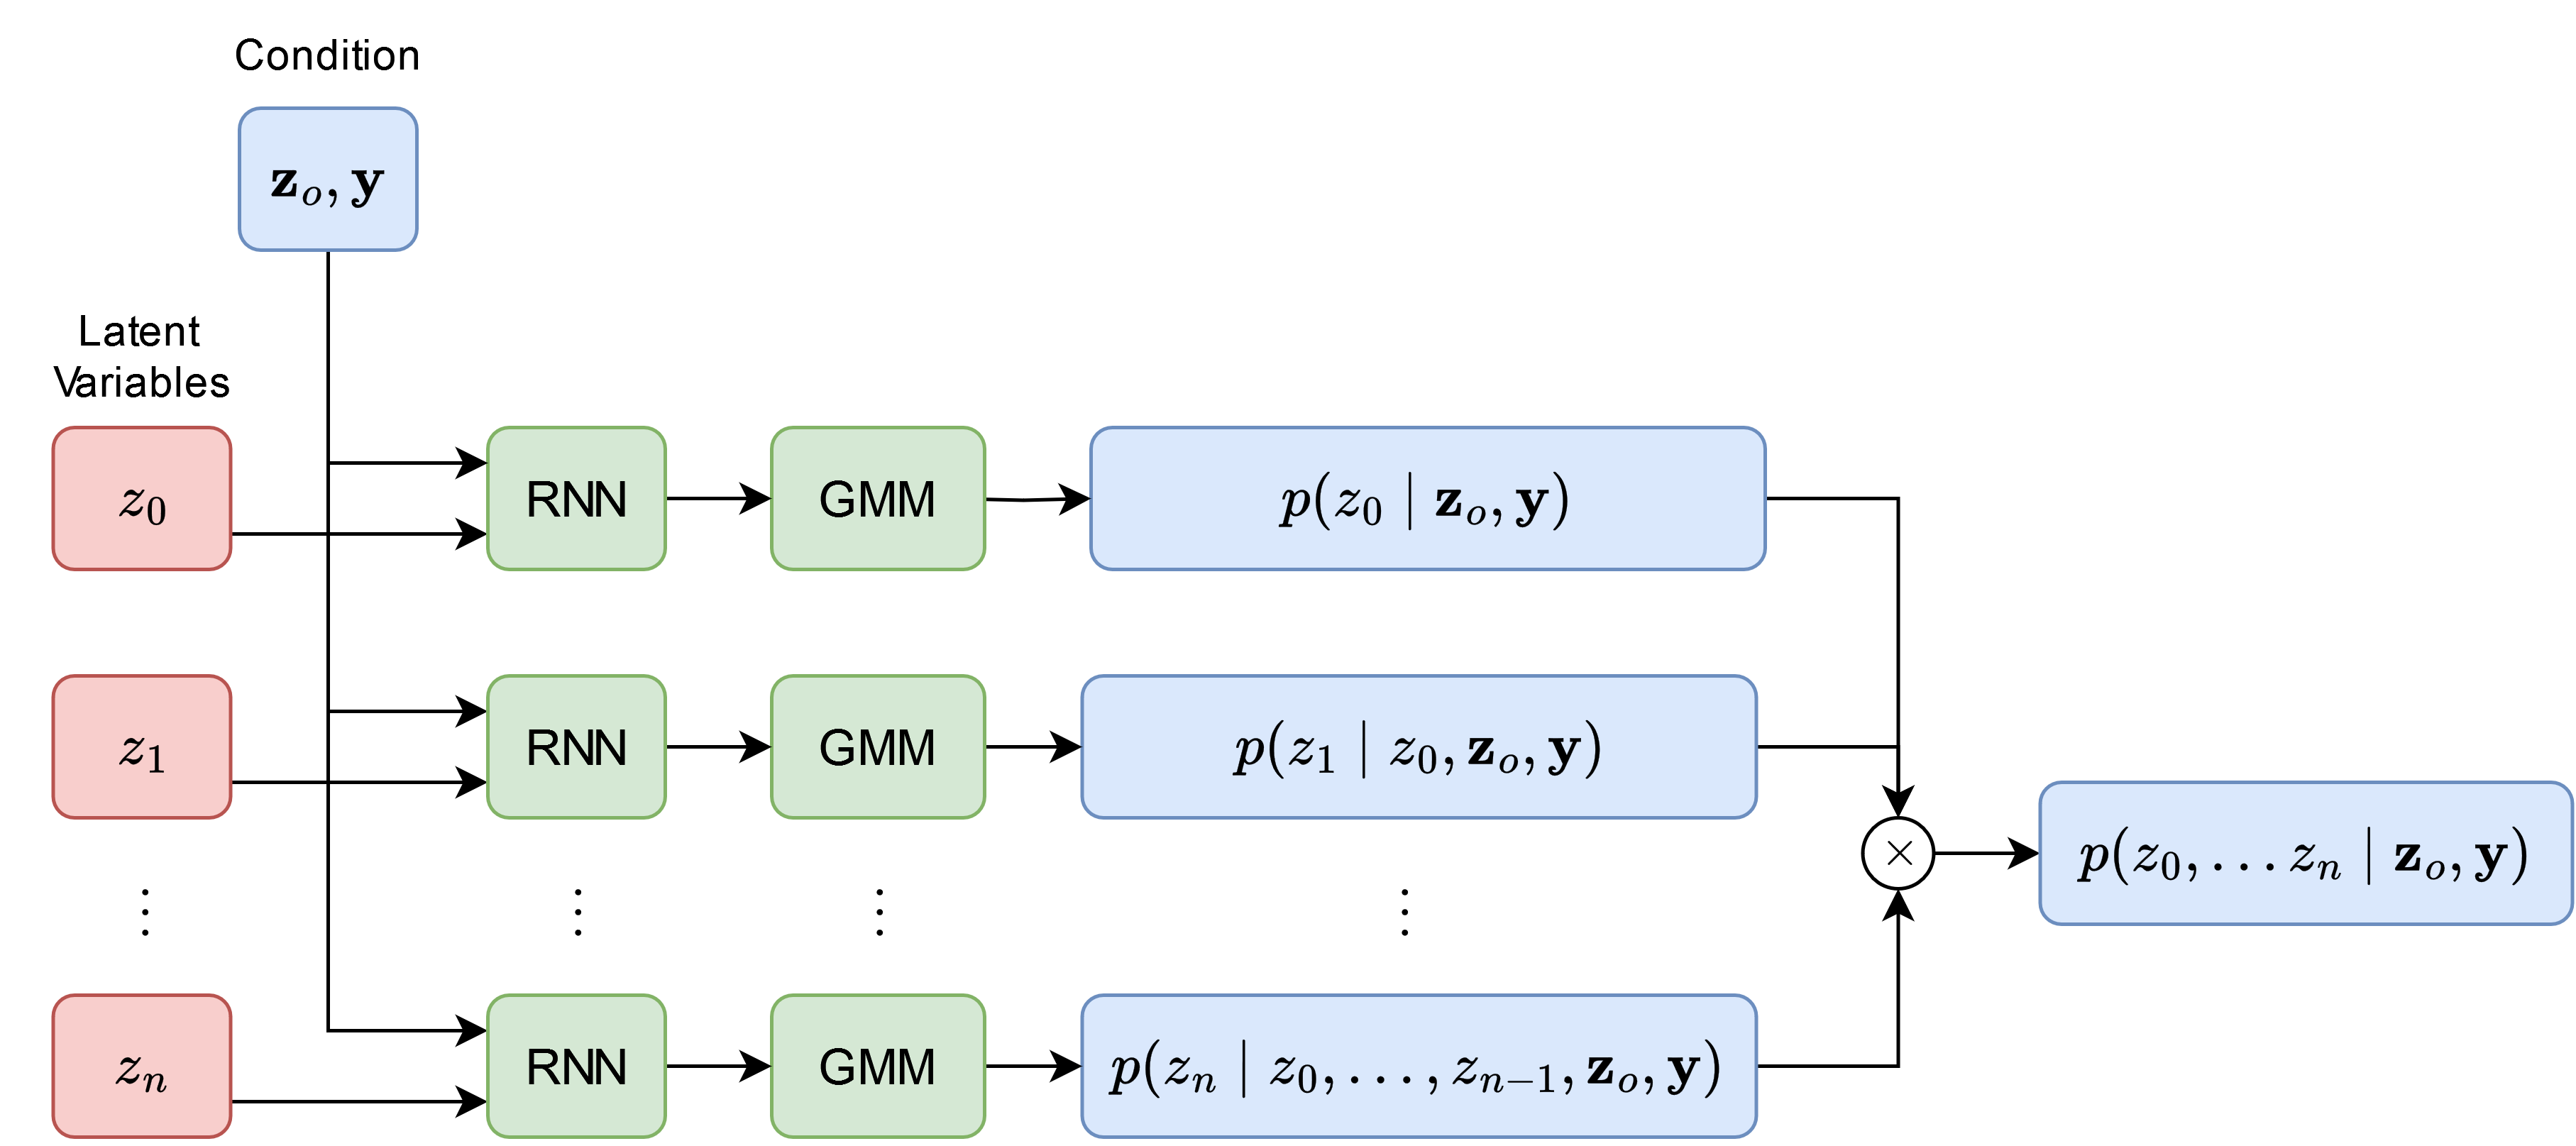
\includegraphics[width=\textwidth]{figs/method/latent-rnn.png}
    \caption{An example of using RNNs and GMMs to model the likelihood $p(z_0, \ldots z_n \mid  \mathbf{z}_o, \mathbf{y})$. The likelihood is conditioned on latent variables corresponding to the intervened concepts $\mathbf{z}_o$, and label $\mathbf{y}.$}
    \label{fig:latent-rnn}
\end{figure}
 

\subsection{Transformations}
In order to transform latent likelihoods $p(z_0, \ldots, z_n \mid \mathbf{z}_o , \mathbf{y})$ to 
the concept likelihoods
$p(c_0,\ldots, c_n \mid \mathbf{c}_o , \mathbf{y})$, we
utilise a set of transformations with learnable parameters that 
map input concepts $c_i$ to latent variables $z_i$. We follow the 
set of conditional transformations defined by Li et al.~\cite{acflow}, and include label $\mathbf{y}$ in the input to make the output likelihoods task-label-specific.
These transformations $q_{\mathbf{c}_o, b, \mathbf{y}}$ are
conditioned on 
intervened concepts $\mathbf{c}_o$, binary mask $b$, and label $\mathbf{y}$, 
and are invertible so that we can obtain the likelihood and 
sample from the latent distribution. 
For all un-intervened concepts $\mathbf{c}_u$,
the transformation maps these concepts to latent variables $q_{\mathbf{c}_o, b, \mathbf{y}}(\mathbf{c}_u) = \mathbf{z}_u$. 
We can then apply the change
of variable theorem from Equation~\ref{equation:change-of-variable} with a conditional extension~\cite{acflow}.
This tells us how to transform 
latent variable likelihoods $p(q_{\mathbf{c}_o, b, \mathbf{y}}(\mathbf{c}_u) \mid \mathbf{c}_o, b, y)$ to concept likelihoods $p(\mathbf{c}_u \mid \mathbf{c}_o, b, y)$.
% \[p(\mathbf{c}_u \mid \mathbf{c}_o, b, y) = \left | 
% \mathop{\mathrm{det}} \frac{d q_{\mathbf{c}_o, b, \mathbf{y}}}{d \mathbf{c}_u}
% \right | p(q_{\mathbf{c}_o, b, \mathbf{y}}(\mathbf{c}_u) \mid \mathbf{c}_o, b, y)\]

In the AC Flow model, we mainly leverage
linear transformations. We use a Multi-Layer Perceptron (MLP)~\cite{feedforward} 
$\phi$ to learn 
a weight matrix $\mathbf{W}$ and bias vector $\mathbf{t}$ that is used to linearly transform a concept vector $\mathbf{c}$. This is a common
technique that transforms concept vectors $\mathbf{c}$ to $\mathbf{z} =\mathbf{W}\mathbf{c} + \mathbf{t}$.
\[\mathbf{W}, \mathbf{t} = \phi(\mathbf{c}_o, b, \mathbf{y})\]
As shown in Figure~\ref{fig:linear-transformation},
this gives us a linear transformation for all concepts $\mathbf{c}$.
However, we only want to transform the un-intervened concepts $\mathbf{c}_u$, as these
are the concepts which we want to obtain the likelihood of. Thus we index the weight and bias vectors to select the entries corresponding to $\mathbf{c}_u$ using the binary mask $b$, where $b$
corresponds to the already intervened concepts $\mathbf{c}_o$. This gives us weight matrix $\mathbf{W}_u$ and bias vector $\mathbf{b}_u$ that can be used to apply a linear transform to $\mathbf{c}_u$.
\[\mathbf{W}_{u} = W[1-b][1-b], \mathbf{b}_{u} = \mathbf{b}[1-b]\]
\[\mathbf{z}_u = \mathbf{W}_{u}\mathbf{c}_u + \mathbf{b}_{u}\]
 This transformation is 
straightforward to invert, and we can find the Jacobian determinant easily and apply the change of variable
theorem to get the likelihood $p(\mathbf{c}_u \mid \mathbf{c}_o, y)$.
Other variants, such as using an RNN to learn linear transformations, are also included to add flexibility to the transformations such that
we are able to model the input data distribution. More details on the transformations
we used can be found in Appendix~\ref{appendix:transformations}.

\begin{figure}[!ht]
    \centering
    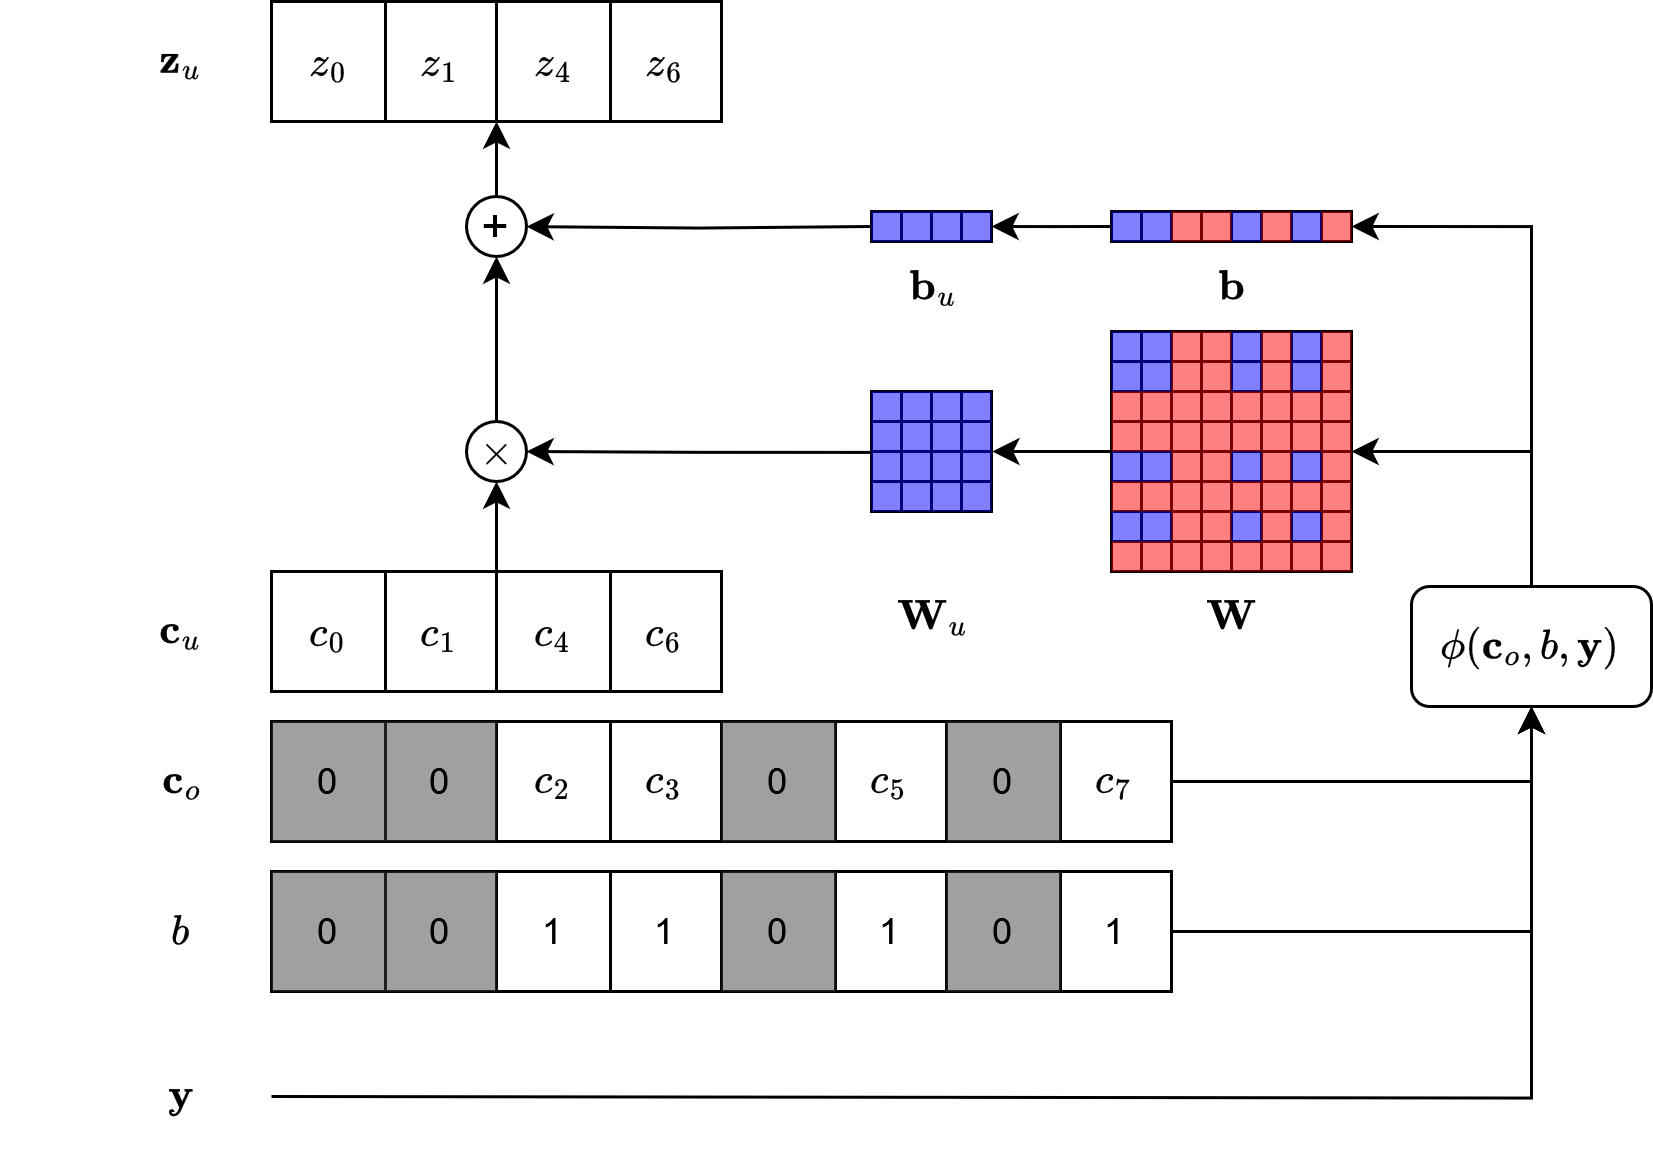
\includegraphics[width=\textwidth]{figs/method/transformations.png}
    \caption{An example of using linear transformations
    in AC Flow models to transform concepts $c_i$ to latent variables $z_i$. The transformation is conditioned on intervened concepts $\mathbf{c}_o$, mask $b$, and label $\mathbf{y}.$}
    \label{fig:linear-transformation}
\end{figure}

These transformations and the latent distribution are both learnt to
approximate the conditional likelihoods $p(c_0, \ldots, c_n \mid \mathbf{y})$
or the likelihood of seeing a set of concepts $p(\mathbf{c}_u \mid \mathbf{y})$.
% seeing a set of unobserved concepts $\mathbf{c}_u$
% given a set of observed concepts $\mathbf{c}_o$ and a class $\mathbf{y}$. 
By using Bayes' theorem, we note that
we can additionally model the conditional likelihoods of the label and un-intervened
concepts
\begin{equation}\label{equation:bayes}
p(\mathbf{y} \mid \mathbf{c}_o ) = \frac{
p( \mathbf{c}_o \mid \mathbf{y}) P(\mathbf{y})}
{\sum_{y'} p( \mathbf{c}_o \mid \mathbf{y}')P(\mathbf{y}')}
\end{equation}
Which the $p(\mathbf{c}_o \mid \mathbf{y})= p(\mathbf{c}_o \mid \emptyset, \mathbf{y})$ terms can be computed from the AC Flow model,
using an empty set of concepts as the condition.
As we can see in Section~\ref{method:rlcem}, this likelihood is used to 
provide rewards to the RL agent. \\ \\
Since the learnt transformations are invertible,
we can also sample from the data distribution
via the underlying distribution.
% Due to the invertible property of the learnt transformations,
% a model learnt this way also allows us to sample from the underlying probability 
% distribution then applying the transformations, which gives us 
% samples from the input distribution.
This is useful for the RL agent to
determine interventions as
it provides information on which concepts are likely to be present 
(or not present) given the currently intervened
concepts. \\ \\
In general, we follow the advised hyperparameters from Li et al.~\cite{acflow}
for building the transformations used in our AC Flow model. This includes the rank of the linear
matrices $\mathbf{W}$ and the hidden dimension of the latent distribution RNN. 
% However, we notice that while
% they use $k \times m$ components in the Gaussian Mixture Model where $k$ is the number of concepts
% and $m$ is the number of classes, we can use $m$ components without any noticeable performance drop.
% Sufficient transformations are required for the AC Flow model to 
% approximate the data distribution accurately, and we do not change them.
\subsection{Training the Surrogate Models}\label{method:training-surrogate-model}
In this project, we adapt AC Flow models to model the likelihoods of concepts in CEMs during interventions.
We follow the description of Li et al.~\cite{afa} and implement corresponding AC Flow models to model
the distribution of concepts. \\ \\
We pre-train the AC Flow model before the CEM or RL agent, after which the pre-trained AC Flow model is frozen (i.e. no longer updated) to use to calculate rewards for the RL agent.
We train the AC Flow models using a combination of two losses, a negative
log likelihood loss and a mean-squared error (MSE) loss . 
Since these models output likelihoods directly,
we can directly maximize the likelihood, or equivalently minimizing the negative log likelihood.
Additionally, a cross entropy loss is incorporated to help the model
learn the conditional likelihood with respect to the label $y$. 
Given $\mathbf{c}_u, \mathbf{c}_o, y$, we compute the class with the highest likelihood
$\hat{y} = \mathop{\mathrm{argmax}}_y p(\mathbf{c}_u, \mathbf{c}_o \mid y)$ and compute 
a cross entropy loss $CE(\hat{y}, y)$ such that the model learns to 
output higher likelihoods for concepts that belong to the correct class.
The loss for training the AC Flow model thus becomes
\begin{equation}\label{equation:ac-flow-loss}
Loss = - \log p(\mathbf{c}_u \mid \mathbf{c}_o, \mathbf{y}) +
 CE(\mathop{\mathrm{argmax}}_\mathbf{y} p(\mathbf{c}_u, \mathbf{c}_o \mid \mathbf{y}),  \mathbf{y})
\end{equation}
In practice, we noticed large likelihood values which
affect the training of the RL agent.
We add a penalty term to the loss to prevent 
the model from outputting large values of likelihoods in general.
To penalize
large values, similar to an $\ell_2$ regularization loss,
we add the square of the logits $\log p(\mathbf{c}_u, \mathbf{c}_o \mid \mathbf{y})$ and 
$\log p(\mathbf{c}_o \mid \mathbf{y})$
to the loss. 
This penalty term is further discussed in 
Section~\ref{eval:surrogate}. 
The final loss for training the
AC Flow model is
\begin{align}
Loss = & - \log p(\mathbf{c}_u \mid \mathbf{c}_o, \mathbf{y}) + 
CE(\mathop{\mathrm{argmax}}_\mathbf{y} p(\mathbf{c}_u, \mathbf{c}_o \mid \mathbf{y}),  \mathbf{y}) \notag
\\ & + \lambda_{\ell_2} \left ( \log^2 p(\mathbf{c}_u, \mathbf{c}_o \mid \mathbf{y}) + 
\log^2 p(\mathbf{c}_o \mid \mathbf{y}) \right )
\label{equation:ac-flow-loss-l2}
\end{align}


\section{RLCEM}\label{method:rlcem}

% Talk about how the RLCEM model is formed
% The goal, losses etc
% Detailed description of what happens during training and testing
% Diagram
% Talk about design choices: num_rollouts, batch_size sampling of budget etc
Instead of using 
the original CBMs as our base models, we adopt CEMs as they have been shown to have
better performance with and without interventions compared to CBMs~\cite{cem}.
Additionally, CEMs are more robust to concept incompleteness, 
which is when the concepts present 
in the dataset annotations do not contain all possible concepts
that can be used to, an important issue in real-life datasets. This is because
CEMs learn to output intermediate
concept embeddings rather than binary values~\cite{cem}.

We construct RLCEMs by augmenting CEMs with an RL agent as 
described below, which is our proposed solution
to a method that learns a non-greedy intervention policy for different budgets.
% We compare our RLCEM against IntCEM and other SOTA intervention policies, which
% are evaluated on the datasets described in~\ref{method:datasets} and we report
% the intervention performance.

\subsection{Training the agent}
% In Active Feature Acquisition as described in Section~\ref{background:afa},
Li et al.~\cite{gsmrl} combine Reinforcement Learning with 
AC Flow models to find the optimal features to acquire 
from the environment in Active Feature Acquisition. We
adopt a similar approach to train the RL agent.

We first pre-train an AC Flow model that learns 
arbitrary conditional likelihoods about the underlying
concepts $p(\mathbf{c}_u \mid \mathbf{c}_o, y)$. 
Then, A Reinforcement Learning agent is trained to maximize 
the reward given in Section~\ref{method:rl}. 
At each
step, the agent is given the current intervened concepts $\mathbf{c}_o$, 
and then the agent samples the next 
concepts to intervene $\mathbf{c}_u$, 
where the agent is rewarded based on the expected information gain
to the target variable.
At each step, the agent has access to the sampled un-intervened concepts $\hat{\mathbf{c}_u}$ 
from the AC Flow model. This allows the RL agent to learn to intervene on concepts that are 
more likely incorrectly predicted.

Compared to Active Feature Acquisition, the problem setting is a lot more complex as
rather than simply acquiring features from the environment, we are trying to determine
which concepts are more likely to be incorrectly predicted by the $\mathbf{x} \to \mathbf{c}$ model, 
and
which concepts are more likely to, when corrected, guide the model towards the correct prediction
 $\mathbf{y}$.
Additionally the goal is to train one RL agent to be able to determine which concepts
to intervene on for different budgets, which adds another layer of complexity as we require
one unified model for the different tasks with different budgets.

\subsection{Reinforcement Learning Algorithm}

As mentioned in Section~\ref{background:rl}, the state-of-the-art RL algorithm 
for learning
a policy is Proximal Policy Optimization (PPO)~\cite{ppo}, which we use
to train a RL agent that learns a non-greedy intervention policy.
PPO utilizes a Critic model to estimate
the value of a particular state, which is the discounted expected future rewards. Then
an Actor model learns a policy
for taking actions that lead to states with higher values as estimated by the
Critic model.

% During training, a state and its true value is computed
% and compared to the estimated value by the Critic, and a value loss is computed to minimize
% the discrepancy between these two values. 
As mentioned in Section~\ref{background:rl},
during training we compute a value loss and a policy loss. The value loss is used to update 
the Critic model to make more accurate estimates of the value of a state, and the policy loss is used to update the Actor model to take actions that lead to better rewards.
% Then a policy loss is computed
% by the discrepancy between actions selected for states and the estimated
% change in value by taking that action.
Ultimately, the Critic model
should be able to estimate the value of a state which reflects its predictive accuracy after all 
future interventions,
and the Actor model should be able to estimate which
interventions lead to the highest label predictive accuracy 
after all interventions.

\subsection{Combining RL with CEM}

Zarlenga et al.~\cite{intcem} showed that combining learning an intervention policy
and learning a CEM as a joint optimization problem achieved the best intervention performance.
Not only do we learn an intervention policy specific to a CEM and task, the 
CEM also learns to be more sensitive to interventions, achieving higher label prediction accuracy
when concepts are intervened. Thus we also combine the training of the RL agent and the CEM
as a joint optimization problem and train
both simultaneously in one training loop.

As shown in Figure~\ref{fig:rlcem}, the training loop
of the RLCEM is as follows:

\begin{enumerate}
    \item The $\mathbf{x} \to \mathbf{c}$ model first computes the predicted concepts $\mathbf{c}$.
    We then compute a weighted concept loss $\mathcal{L}_{\text{concept}}$ with the true concepts to train the $\mathbf{x} \to \mathbf{c}$ model.
    \item Since we want to train the RL agent $\mathcal{A}$ to be able to learn 
    the concepts to intervene for different budgets, thus during training 
    for each mini-batch, we sample $n_{\text{rollout}}$ different budgets.

    For each sampled budget $T$, 
    in each step $t$
    the RL environment $\mathcal{E}$ provides
    the states $\textbf{obs}^t$, the remaining budget $T - t$, 
    and the previous reward $r^{t-1}$ to the RL agent. The agent then samples actions
    $\hat{a}^{(t)}$, which are then used to update the intervention mask $\bm{\mu}^{t+1}$
    and the predicted concepts $\hat{\mathbf{c}}^{t+1}$ in the next step.

    \item After all interventions are performed, the states $\textbf{obs}$,
    actions $\hat{a}$,
    the corresponding rewards $r$, are used to calculate the true values of states.
    This is then compared against the values estimated by the Critic model
    $\hat{V}(\textbf{obs})$
    to compute a value loss $\mathcal{L}_{\text{value}}$ for the Critic model.
    Then the estimated values $\hat{V}(\textbf{obs})$ and the estimated 
    next state values $\hat{Q}(\textbf{obs}, \hat{a}, r)$
    are used to compute the advantage function $\hat{A}$ which tells us
    the advantage of taking actions. These advantages are then used to compute
    a policy loss $\mathcal{L}_{\text{policy}}$ to update the Actor model.
    These two losses combine to give us the intervention loss $\mathcal{L}_{\text{intervention}}$.
    \item Lastly, we compute label losses for 
    updating 
    the $\mathbf{c} \to \mathbf{y}$ model using concepts before intervention and after intervention. These losses are
    discounted by $\gamma^T$, similar to IntCEM. The sum of these losses give us a weighted label loss $\mathcal{L}_{\text{label}}$ to train the $\mathbf{c} \to \mathbf{y}$ model.
\end{enumerate}

\begin{figure}
    \centering
    \includegraphics*[width=\textwidth]{figs/method/rlcem.png}
    \caption{The training loop of RLCEM. $T$ is a sampled budget for training, $\mathcal{E}$ is the RL environment, $\mathcal{A}$ the RL agent, 
    and $\hat{V}, \hat{Q}$ the estimated value functions from the agent. 1. The CEM predicts concept embeddings $\mathbf{e}$
    which is used to compute a  concept loss $\mathcal{L}_{\text{concept}}$ to update the concept predictor model $g$.
    2. For a budget $T$, The RL Agent sequentially samples actions $\hat{a}^(t)$ for states $\textbf{obs}^{t-1}$, which are then used to compute interventions and transition to a new state $\textbf{obs}^{t}$. We repeat this until we use up the budget.
    3. The states $\textbf{obs}^{t}$, actions $\hat{a}^{t}$, and rewards $r^{t}$ are used to compute an intervention loss $\mathcal{L}_{\text{intervention}}$ to update the RL agent. 4. We compute label loss $\mathcal{L}_{\text{label}}$ using the intervened concepts $\hat{\mathbf{c}}^t$ to update the label predictor model $f$.
    }
    \label{fig:rlcem}
\end{figure}

The structure of the training loop is similar to IntCEM.
 We compute a concept loss
and a label loss without interventions.
Then we sample interventions according to our intervention policy model,
and compute label losses with respect to the intervened concepts to increase 
the CEM's sensitivty to interventions. Then we update our intervention policy
model so that it makes better interventions which lead to a higher accuracy.
Similar to IntCEM's loss equation in~\ref{equation:intcem-loss}, the final loss for training the model is given by 
\[\mathcal{L} = \lambda_{\text{concept}} \mathcal{L}_{\text{concept}}
+  \lambda_{\text{label}} \mathcal{L}_{\text{label}}
+  \lambda_{\text{intervention}} \mathcal{L}_{\text{intervention}}\]

\subsection{Limitations}\label{method:limitations}

A major concern is the Time Complexity associated with learning
such an RLCEM. As mentioned in~\ref{method:rl}, in order to ensure
that the RL agent learns a policy for a variety of different budgets,
for $k$ concepts and $n$ concept groups,
 we sample $O(n)$ different policies for each mini-batch during training, set 
to $n/2$ in practice. For each budget, the RL agent needs to sample
$O(n)$ actions and compute the corresponding rewards used for training. 
Compared to
a greedy intervention policy which is trained sequentially over
$n$ possible interventions, 
a non-greedy intervention policy learnt using
RL requires more complexity of $O(n^2)$ compared to $O(n)$.
Additionally, since the underlying surrogate model utilises a sequential
RNN to model the conditional distribution which has time complexity
proportional to the number of concepts $O(k)$, the final 
time complexity can reach up to $O(n^2k)$ compared to $O(n)$ of the current
greedy intervention policy methods which adds a lot of cost to training.
This limitation
and its impacts
are further discussed in Section~\ref{eval:limitations}.\\

\section{Summary}
In this chapter, we presented a new method 
that utilises Reinforcement Learning
to learn a non-greedy intervention policy,
along with how we propose 
to train a generative AC Flow model to
provide intermediate rewards to the RL agent during
training and testing to guide its intervention decisions.
This allows us to
develop a method to find non-greedy intervention policies for different budgets.
In the next chapter, we evaluate the performance of the proposed
RLCEM against current methods on how
they perform with and without interventions.

 % In this chapter we presented a new method, in the next chapter we evaluate etc etc
 % be explicit, announce what you're saying eg. this chapter, next chapter, the research question 

 % datasets goes to evaluation
 % baseline etc
 % 
\end{document}